\documentclass[11pt]{article}
\usepackage[margin=1in]{geometry}
\usepackage{hyperref}
\usepackage{enumitem}
\usepackage{listings}
\usepackage{amsmath}
\usepackage{amssymb}
\usepackage{xcolor}
\usepackage{tikz}
\usetikzlibrary{arrows.meta, positioning, shapes.geometric, fit, backgrounds}
\usepackage{subcaption}

% Type formatting commands
\newcommand{\ttype}[1]{\mathsf{#1}}
\newcommand{\tfield}[1]{\mathit{#1}}
\newcommand{\tkw}[1]{\textbf{#1}}
\newcommand{\tcomment}[1]{\textcolor{gray}{\textit{#1}}}

\lstset{
  basicstyle=\ttfamily\footnotesize,
  keywordstyle=\bfseries,
  frame=single,
  framerule=0.3pt,
  columns=flexible,
  keepspaces=true,
  showstringspaces=false,
  aboveskip=0.8em,
  belowskip=0.8em,
  mathescape=true,
  literate={->}{$\rightarrow$}{2} {=>}{$\Rightarrow$}{2}
}

\title{Rewatch: Core Algorithms for Incremental Compilation}
\author{}
\date{}

\begin{document}
\maketitle

\begin{abstract}
Rewatch is the build and watch engine for ReScript projects. This document presents its core algorithms as typed functions, abstracting away implementation details to expose the fundamental computational patterns. The goal is to identify algorithmic building blocks that could be expressed using incremental and reactive computation primitives.
\end{abstract}

\section{Introduction}

A build system for a typed language must solve several interrelated problems:
\begin{enumerate}[noitemsep]
  \item \textbf{Discovery}: Find source files and compute a package dependency graph.
  \item \textbf{Parsing}: Transform source files into abstract syntax trees.
  \item \textbf{Dependency Analysis}: Extract module-level dependencies from parsed sources.
  \item \textbf{Compilation}: Compile modules in dependency order, respecting the constraint that a module's interface must be available before its dependents compile.
  \item \textbf{Incrementality}: When inputs change, recompute only what is necessary.
\end{enumerate}

The key insight is that these problems decompose into a small set of computational patterns: \emph{graph construction}, \emph{fixpoint computation}, \emph{topological scheduling}, and \emph{change propagation}. We present each phase as a pure function with explicit inputs and outputs, then discuss how dirtiness flows through the system.

\section{Build Flows Overview}

Before diving into the details, we present the two main execution flows: one-shot build and watch mode.

\begin{figure}[ht]
\centering

% --- Subfigure (a): One-shot build ---
\begin{subfigure}[b]{\textwidth}
\centering
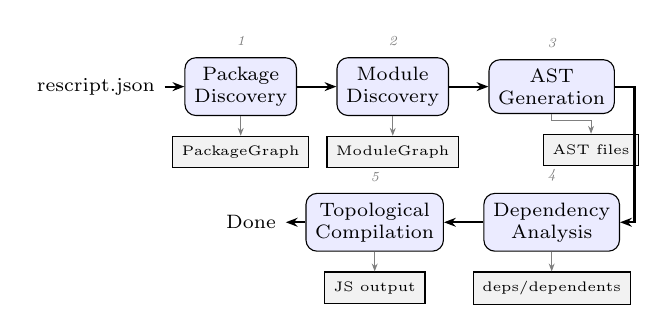
\begin{tikzpicture}[
    node distance=0.4cm and 0.5cm,
    phase/.style={rectangle, draw, rounded corners, minimum width=1.4cm, minimum height=0.6cm, align=center, fill=blue!8, font=\scriptsize},
    data/.style={rectangle, draw, minimum width=1.2cm, minimum height=0.4cm, align=center, fill=gray!10, font=\tiny},
    arrow/.style={-{Stealth[length=1.5mm]}, thick},
    label/.style={font=\tiny\itshape, text=gray}
]

% Row 1: First three phases
\node[phase] (pkg) {Package\\Discovery};
\node[phase, right=of pkg] (mod) {Module\\Discovery};
\node[phase, right=of mod] (parse) {AST\\Generation};

% Row 2: Last two phases
\node[phase, below=1.0cm of parse] (deps) {Dependency\\Analysis};
\node[phase, left=of deps] (compile) {Topological\\Compilation};

% Data stores
\node[data, below=0.25cm of pkg] (pkgdata) {PackageGraph};
\node[data, below=0.25cm of mod] (moddata) {ModuleGraph};
\node[data, below=0.25cm of parse, xshift=0.5cm] (astdata) {AST files};
\node[data, below=0.25cm of deps] (depdata) {deps/dependents};
\node[data, below=0.25cm of compile] (outdata) {JS output};

% Input/Output
\node[left=0.25cm of pkg, font=\scriptsize] (input) {rescript.json};
\node[left=0.25cm of compile, font=\scriptsize] (output) {Done};

% Arrows - top row
\draw[arrow] (input) -- (pkg);
\draw[arrow] (pkg) -- (mod);
\draw[arrow] (mod) -- (parse);

% Arrow turning down
\draw[arrow] (parse.east) -- ++(0.25,0) |- (deps.east);

% Bottom row
\draw[arrow] (deps) -- (compile);
\draw[arrow] (compile) -- (output);

% Arrows to data
\draw[-{Stealth[length=1mm]}, gray] (pkg) -- (pkgdata);
\draw[-{Stealth[length=1mm]}, gray] (mod) -- (moddata);
\draw[-{Stealth[length=1mm]}, gray] (parse.south) -- ++(0,-.08) -| (astdata);
\draw[-{Stealth[length=1mm]}, gray] (deps) -- (depdata);
\draw[-{Stealth[length=1mm]}, gray] (compile) -- (outdata);

% Labels
\node[label, above=0.02cm of pkg] {1};
\node[label, above=0.02cm of mod] {2};
\node[label, above=0.02cm of parse] {3};
\node[label, above=0.02cm of deps] {4};
\node[label, above=0.02cm of compile] {5};

\end{tikzpicture}
\caption{One-shot build: phases 1--3 discover and parse; phases 4--5 analyze and compile.}
\label{fig:oneshot}
\end{subfigure}

\vspace{0.4cm}

% --- Subfigure (b): Watch mode ---
\begin{subfigure}[b]{\textwidth}
\centering
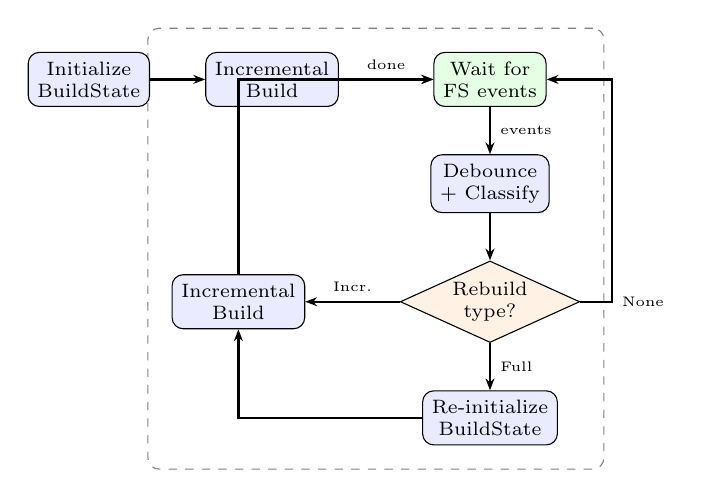
\begin{tikzpicture}[
    node distance=0.6cm and 0.8cm,
    phase/.style={rectangle, draw, rounded corners, minimum width=1.4cm, minimum height=0.55cm, align=center, fill=blue!8, font=\scriptsize},
    decision/.style={diamond, draw, aspect=2.2, align=center, fill=orange!10, inner sep=1pt, font=\scriptsize},
    event/.style={rectangle, draw, rounded corners, minimum width=1.3cm, minimum height=0.5cm, align=center, fill=green!10, font=\scriptsize},
    arrow/.style={-{Stealth[length=1.5mm]}, thick},
    label/.style={font=\tiny, text=black}
]

% Initial build (left side)
\node[phase] (init) {Initialize\\BuildState};
\node[phase, right=0.7cm of init] (fullbuild) {Incremental\\Build};

% Event loop - vertical stack
\node[event, right=1.2cm of fullbuild] (wait) {Wait for\\FS events};
\node[phase, below=0.6cm of wait] (debounce) {Debounce\\+ Classify};
\node[decision, below=0.6cm of debounce] (decide) {Rebuild\\type?};

% Rebuild paths
\node[phase, left=1.2cm of decide] (incr) {Incremental\\Build};
\node[phase, below=0.6cm of decide] (reinit) {Re-initialize\\BuildState};

% Arrows - main flow
\draw[arrow] (init) -- (fullbuild);
\draw[arrow] (fullbuild) -- node[above, label] {done} (wait);

% Event loop vertical
\draw[arrow] (wait) -- node[right, label] {events} (debounce);
\draw[arrow] (debounce) -- (decide);

% Decision branches
\draw[arrow] (decide.west) -- node[above, label] {Incr.} (incr.east);
\draw[arrow] (decide.south) -- node[right, label] {Full} (reinit.north);

% None branch
\draw[arrow] (decide.east) -- ++(0.4,0) node[right, label] {None} |- (wait.east);

% Return paths
\draw[arrow] (incr.north) |- (wait.west);
\draw[arrow] (reinit.west) -| (incr.south);

% Background for event loop
\begin{scope}[on background layer]
\node[draw=gray, dashed, rounded corners, fit=(wait)(debounce)(decide)(incr)(reinit), inner sep=0.3cm, label={[font=\tiny\itshape, text=gray]above:Event Loop}] {};
\end{scope}

\end{tikzpicture}
\caption{Watch mode: event loop triggers incremental or full rebuilds based on file changes.}
\label{fig:watch}
\end{subfigure}

\caption{Build flows. (a) One-shot build executes phases sequentially, producing intermediate data (gray boxes). (b) Watch mode wraps the build in an event loop; content changes trigger incremental rebuilds, structural changes trigger full re-initialization.}
\label{fig:flows}
\end{figure}

\subsection{One-Shot Build}

A one-shot build (Figure~\ref{fig:oneshot}) executes phases sequentially: package discovery, module discovery, AST generation, dependency analysis, and topological compilation. Each phase produces data consumed by subsequent phases.

\subsection{Watch Mode}

Watch mode (Figure~\ref{fig:watch}) wraps the pipeline in an event loop. After an initial build, the system monitors file changes. Content changes mark modules dirty for incremental rebuild; structural changes (file creation/deletion) trigger full re-initialization.

\subsection{Key Data Flow Insight}

The central invariant is that the \emph{ModuleGraph} persists across incremental rebuilds in watch mode, with dirty bits controlling which computations are re-executed. This is the essence of incrementality: rather than recomputing everything, we track what changed and propagate dirtiness through the dependency graph.

\section{Type Vocabulary}

We define a vocabulary of types to describe the state space of the build system. These types abstract over file system paths and other implementation details.

\subsection{Identifiers and Paths}

We begin with primitive types representing identifiers and content fingerprints:
\[
\begin{array}{l@{\quad}l}
\ttype{Path} & \tcomment{Canonical absolute file path} \\
\ttype{ModuleName} & \tcomment{Logical module identifier (e.g., ``List'', ``MyApp\text{-}Utils'')} \\
\ttype{PackageName} & \tcomment{Package identifier (from rescript.json)} \\
\ttype{Hash} & \tcomment{Content hash for change detection} \\
\ttype{Timestamp} & \tcomment{File modification time}
\end{array}
\]

\subsection{Source Representation}

A source module consists of an implementation file and an optional interface file. Each file carries metadata for tracking changes.

\medskip
\noindent\textbf{File metadata:}
\[
\ttype{FileInfo} = \left\{
\begin{array}{l@{\;:\;}l@{\quad}l}
\tfield{path} & \ttype{Path} \\
\tfield{lastModified} & \ttype{Timestamp} \\
\tfield{parseDirty} & \ttype{Bool} & \tcomment{needs re-parsing?} \\
\tfield{parseState} & \ttype{ParseState} & \tcomment{Pending $\mid$ Success $\mid$ Warning $\mid$ Error}
\end{array}
\right\}
\]

\medskip
\noindent\textbf{Source file pair:}
\[
\ttype{SourceFile} = \left\{
\begin{array}{l@{\;:\;}l}
\tfield{implementation} & \ttype{FileInfo} \\
\tfield{interface} & \ttype{Option}\langle\ttype{FileInfo}\rangle
\end{array}
\right\}
\]

\medskip
\noindent\textbf{Source type (sum type):}
\[
\ttype{SourceType} ::= \ttype{Source}(\ttype{SourceFile}) \mid \ttype{MlMap}
\]
where $\ttype{Source}$ represents a regular \texttt{.res}/\texttt{.resi} pair and $\ttype{MlMap}$ represents a namespace alias file.

\subsection{Module Graph}

The central data structure is a directed graph of modules with dependency edges.

\[
\ttype{Module} = \left\{
\begin{array}{l@{\;:\;}l@{\quad}l}
\tfield{name} & \ttype{ModuleName} \\
\tfield{package} & \ttype{PackageName} \\
\tfield{source} & \ttype{SourceType} \\
\tfield{deps} & \mathcal{P}(\ttype{ModuleName}) & \tcomment{modules this depends on} \\
\tfield{dependents} & \mathcal{P}(\ttype{ModuleName}) & \tcomment{modules depending on this} \\
\tfield{compileDirty} & \ttype{Bool} & \tcomment{needs recompilation?} \\
\tfield{depsDirty} & \ttype{Bool} & \tcomment{dependency set changed?} \\
\tfield{lastCmiHash} & \ttype{Option}\langle\ttype{Hash}\rangle & \tcomment{ABI fingerprint}
\end{array}
\right\}
\]

The module graph is a map from names to modules:
\[
\ttype{ModuleGraph} = \ttype{ModuleName} \rightharpoonup \ttype{Module}
\]

\subsection{Package Structure}

Packages group modules and declare inter-package dependencies.

\[
\ttype{Package} = \left\{
\begin{array}{l@{\;:\;}l@{\quad}l}
\tfield{name} & \ttype{PackageName} \\
\tfield{path} & \ttype{Path} \\
\tfield{namespace} & \ttype{Option}\langle\ttype{String}\rangle \\
\tfield{deps} & \mathcal{P}(\ttype{PackageName}) & \tcomment{declared dependencies} \\
\tfield{devDeps} & \mathcal{P}(\ttype{PackageName}) & \tcomment{dev-only dependencies} \\
\tfield{sourceFiles} & \ttype{Path} \rightharpoonup \ttype{SourceMeta} \\
\tfield{modules} & \mathcal{P}(\ttype{ModuleName})
\end{array}
\right\}
\]

\[
\ttype{PackageGraph} = \ttype{PackageName} \rightharpoonup \ttype{Package}
\]

\subsection{Build State}

The complete build state combines packages, modules, and compiler metadata.

\[
\ttype{BuildState} = \left\{
\begin{array}{l@{\;:\;}l}
\tfield{packages} & \ttype{PackageGraph} \\
\tfield{modules} & \ttype{ModuleGraph} \\
\tfield{moduleNames} & \mathcal{P}(\ttype{ModuleName}) \\
\tfield{compilerHash} & \ttype{Hash} \\
\tfield{depsInitialized} & \ttype{Bool}
\end{array}
\right\}
\]

\section{Phase 1: Package Discovery}

The first phase discovers packages and constructs the package dependency graph. This is a recursive traversal of the file system following dependency declarations.

\subsection{Specification}

\begin{lstlisting}
readDependencies : (PackageName, Path) -> List<Package>
\end{lstlisting}

Given a package name and its path, return all transitive dependencies. The algorithm must handle cycles in the dependency graph (which indicate an error).

\subsection{Algorithm}

\begin{lstlisting}
readDependencies(name, path):
  config = readConfig(path)
  declared = config.dependencies $\cup$ config.devDependencies
  result = []
  for depName in declared:
    if depName $\notin$ visited:
      visited.add(depName)
      depPath = resolvePath(depName, path)
      result.append(Package(depName, depPath, readConfig(depPath)))
      result.extend(readDependencies(depName, depPath))
  return result
\end{lstlisting}

\textbf{Pattern}: This is a \emph{depth-first graph traversal} with memoization to handle shared dependencies. The visited set ensures each package is processed once.

\subsection{Package Graph Construction}

\begin{lstlisting}
makePackages : Path -> PackageGraph

makePackages(root):
  rootPkg = makePackage(readConfig(root), root, isRoot=true)
  deps = flattenDependencies(readDependencies(rootPkg.name, root))
  packages = { rootPkg.name: rootPkg }
  for dep in deps:
    packages[dep.name] = makePackage(dep.config, dep.path, isRoot=false)
  return packages
\end{lstlisting}

\section{Phase 2: Module Discovery}

Once packages are known, we enumerate source files and construct the initial module graph.

\subsection{Specification}

\begin{lstlisting}
discoverModules : PackageGraph -> ModuleGraph

discoverModules(packages):
  modules = {}
  for pkg in packages.values():
    for (path, meta) in pkg.sourceFiles:
      moduleName = pathToModuleName(path, pkg.namespace)
      modules[moduleName] = Module {
        name = moduleName,
        package = pkg.name,
        source = makeSourceType(path, meta),
        deps = $\emptyset$,
        dependents = $\emptyset$,
        compileDirty = true,
        depsDirty = true,
        lastCmiHash = None
      }
  return modules
\end{lstlisting}

\textbf{Pattern}: This is a \emph{map} operation over packages, flattened into a single module namespace. Namespace handling ensures module names are unique across packages.

\section{Phase 3: AST Generation (Parsing)}

Parsing transforms source files into ASTs. This phase runs in parallel for independent modules and tracks dirtiness.

\subsection{Specification}

\begin{lstlisting}
generateAsts : ModuleGraph -> (ModuleGraph, List<Error>)
\end{lstlisting}

For each module whose source is \texttt{parseDirty}, invoke the parser. Update parse state and propagate dirtiness to compilation.

\subsection{Algorithm}

\begin{lstlisting}
generateAsts(modules):
  errors = []
  results = parallel for (name, m) in modules:
    if isParseDirty(m):
      (astPath, err) = parse(m.source.implementation.path)
      (iastPath, ierr) = if m.source.interface then
                           parse(m.source.interface.path)
                         else (None, None)
      yield (name, astPath, iastPath, err $\cup$ ierr)
    else:
      yield (name, cachedAstPath(m), cachedIastPath(m), $\emptyset$)
  
  for (name, ast, iast, errs) in results:
    modules[name].source.implementation.parseDirty = false
    modules[name].source.interface?.parseDirty = false
    if errs $\neq$ $\emptyset$:
      modules[name].source.implementation.parseState = Error
      errors.extend(errs)
    else:
      modules[name].compileDirty = true  -- propagate to compilation
      modules[name].depsDirty = true     -- deps may have changed
  
  return (modules, errors)
\end{lstlisting}

\textbf{Pattern}: This is a \emph{parallel map} with \emph{dirty-tracking}. The key invariant is: if a source file changed, its AST must be regenerated, and downstream phases (dependency analysis, compilation) must be notified.

\section{Phase 4: Dependency Discovery}

Dependencies are extracted from AST files. Each AST file contains a header listing the modules it imports.

\subsection{Specification}

\begin{lstlisting}
computeDependencies : ModuleGraph -> ModuleGraph
\end{lstlisting}

For each module with \texttt{depsDirty = true}, read its dependency set from the AST. Update both \texttt{deps} and \texttt{dependents} to maintain the bidirectional graph.

\subsection{Algorithm}

\begin{lstlisting}
computeDependencies(modules, validModules):
  newDeps = parallel for (name, m) in modules:
    if m.depsDirty:
      rawDeps = readDepsFromAst(m.astPath)
      deps = normalizeNamespace(rawDeps, m.package.namespace)
      deps = filterValid(deps, validModules, m.package.allowedDeps)
      yield (name, deps)
    else:
      yield (name, m.deps)
  
  -- Update dependency graph (sequential for consistency)
  for (name, deps) in newDeps:
    oldDeps = modules[name].deps
    modules[name].deps = deps
    modules[name].depsDirty = false
    
    -- Update dependents for added/removed edges
    for d in (deps $\setminus$ oldDeps):
      modules[d].dependents.add(name)
    for d in (oldDeps $\setminus$ deps):
      modules[d].dependents.remove(name)
  
  return modules
\end{lstlisting}

\textbf{Pattern}: This is a \emph{graph edge computation} with \emph{incremental update}. The bidirectional edges (deps/dependents) enable efficient traversal in both directions—forward for compilation order, backward for dirty propagation.

\section{Phase 5: Incremental Compilation}

Compilation is the most complex phase. It must respect the constraint that a module cannot compile until all its dependencies are compiled, and it must propagate changes when a module's interface (ABI) changes.

\subsection{The Compile Universe}

Not every module needs consideration during compilation—only those that are dirty or transitively depend on dirty modules. We call this the \emph{compile universe}.

\begin{lstlisting}
computeCompileUniverse : ModuleGraph -> Set<ModuleName>

computeCompileUniverse(modules):
  dirty = { name | (name, m) $\in$ modules, m.compileDirty }
  universe = dirty
  frontier = dirty
  while frontier $\neq$ $\emptyset$:
    newFrontier = $\emptyset$
    for name in frontier:
      for dep in modules[name].dependents:
        if dep $\notin$ universe:
          universe.add(dep)
          newFrontier.add(dep)
    frontier = newFrontier
  return universe
\end{lstlisting}

\textbf{Pattern}: This is a \emph{forward reachability} computation—a breadth-first traversal along the dependents edges, starting from the dirty set.

\subsection{Topological Compilation}

Within the compile universe, modules must be compiled in dependency order. Modules with no pending dependencies can compile in parallel.

\begin{lstlisting}
compile : (ModuleGraph, Set<ModuleName>) -> (ModuleGraph, List<Error>)

compile(modules, universe):
  compiled = $\emptyset$
  errors = []
  
  -- Ready set: modules whose deps are all outside universe or compiled
  ready = { m $\in$ universe | modules[m].deps $\cap$ universe $\subseteq$ compiled }
  
  while ready $\neq$ $\emptyset$:
    results = parallel for name in ready:
      m = modules[name]
      if not m.compileDirty:
        yield (name, Ok, unchanged=true)
      else:
        oldHash = computeCmiHash(m)
        err = compileModule(m)
        newHash = computeCmiHash(m)
        yield (name, err, unchanged=(oldHash = newHash))
    
    for (name, result, unchanged) in results:
      compiled.add(name)
      ready.remove(name)
      
      if result is Error:
        errors.append(result)
      else:
        modules[name].compileDirty = false
        
        -- ABI change propagation
        if not unchanged:
          for dep in modules[name].dependents:
            modules[dep].compileDirty = true
            modules[dep].depsDirty = true
      
      -- Add newly ready modules
      for dep in modules[name].dependents:
        if dep $\in$ universe and dep $\notin$ compiled:
          if modules[dep].deps $\cap$ universe $\subseteq$ compiled:
            ready.add(dep)
    
    if ready = $\emptyset$ and compiled $\neq$ universe:
      -- Cycle detected
      cycle = findCycle(universe $\setminus$ compiled, modules)
      errors.append(CycleError(cycle))
      break
  
  return (modules, errors)
\end{lstlisting}

\textbf{Patterns}: This algorithm combines several patterns:
\begin{itemize}[noitemsep]
  \item \textbf{Topological scheduling}: Processing nodes level-by-level based on dependency constraints.
  \item \textbf{ABI fingerprinting}: Comparing interface hashes to detect meaningful changes.
  \item \textbf{Backward change propagation}: When an interface changes, dependents are marked dirty for recompilation.
  \item \textbf{Cycle detection}: Identifying strongly connected components that cannot be compiled.
\end{itemize}

\subsection{ABI Change Propagation}

The crucial insight for incrementality is that not all recompilations require recompiling dependents. If a module's implementation changes but its interface (`.cmi` file) does not, dependents need not recompile. We track this via content hashing:

\begin{lstlisting}
propagateDirtiness : (ModuleName, Bool, ModuleGraph) -> ModuleGraph

propagateDirtiness(name, abiChanged, modules):
  if abiChanged:
    for dep in modules[name].dependents:
      modules[dep].compileDirty = true
      modules[dep].depsDirty = true
  return modules
\end{lstlisting}

\section{Phase 6: Watch Mode and Event Processing}

In watch mode, the build system responds to file system changes. Events are batched and debounced before triggering a rebuild.

\subsection{Event Classification}

File system events are classified by their effect on the build:
\[
\ttype{FsEvent} ::= \ttype{Modified}(\ttype{Path}) \mid \ttype{Created}(\ttype{Path}) \mid \ttype{Deleted}(\ttype{Path}) \mid \ttype{Renamed}(\ttype{Path} \times \ttype{Path})
\]

The rebuild decision is a three-valued type:
\[
\ttype{RebuildType} ::= \ttype{Incremental} \mid \ttype{Full} \mid \ttype{None}
\]

\subsection{Event Processing}

\begin{lstlisting}
processEvents : (List<FsEvent>, ModuleGraph) -> (ModuleGraph, RebuildType)

processEvents(events, modules):
  rebuildType = None
  for event in events:
    path = eventPath(event)
    if not isRescriptFile(path): continue
    if isInBuildDir(path): continue
    
    case event of:
      Modified(path):
        moduleName = pathToModule(path, modules)
        modules[moduleName].source.implementation.parseDirty = true
        rebuildType = max(rebuildType, Incremental)
      
      Created(path) | Deleted(path) | Renamed(_):
        -- Structural change requires full rebuild
        rebuildType = Full
  
  return (modules, rebuildType)
\end{lstlisting}

\textbf{Pattern}: Event processing is a \emph{fold} over events, accumulating both state changes and a rebuild decision. The key distinction is between content changes (incremental) and structural changes (full rebuild).

\subsection{Watch Loop}

\begin{lstlisting}
watchLoop : (Path, BuildState) -> $\bot$  -- runs forever

watchLoop(root, state):
  loop:
    events = debounce(drainEventQueue(), 50ms)
    (modules, rebuildType) = processEvents(events, state.modules)
    state.modules = modules
    
    case rebuildType of:
      None -> sleep(50ms)
      
      Incremental ->
        state = incrementalBuild(state)
      
      Full ->
        state = initializeBuild(root)
        state = incrementalBuild(state)
\end{lstlisting}

\section{Summary of Computational Patterns}

The algorithms in Rewatch decompose into a small set of reusable patterns:

\begin{center}
\begin{tabular}{|l|l|l|}
\hline
\textbf{Pattern} & \textbf{Where Used} & \textbf{Character} \\
\hline
Graph traversal (DFS/BFS) & Package discovery, universe expansion & Pure \\
Parallel map & AST generation, dep extraction & Pure, parallelizable \\
Incremental graph update & Dependency edge maintenance & Stateful \\
Topological scheduling & Compilation order & Stateful \\
Content hashing & ABI change detection & Pure \\
Dirty bit propagation & Change notification & Stateful \\
Event folding & Watch mode & Stateful \\
Debouncing & Event batching & Time-aware \\
\hline
\end{tabular}
\end{center}

\section{Towards Reactive/Incremental Formulation}

The patterns identified above suggest natural mappings to incremental computation frameworks:

\begin{itemize}[noitemsep]
  \item \textbf{Dependency tracking}: The \texttt{deps}/\texttt{dependents} bidirectional graph is essentially a dependency graph that incremental frameworks maintain automatically.
  
  \item \textbf{Dirty propagation}: Marking dependents dirty when a module changes is the core operation of demand-driven incremental computation (self-adjusting computation).
  
  \item \textbf{ABI fingerprinting}: Comparing old and new values before propagating changes corresponds to ``cutoff'' in incremental frameworks—avoiding unnecessary downstream recomputation when values are equal.
  
  \item \textbf{Topological compilation}: The level-by-level processing with ready-set tracking mirrors how incremental frameworks schedule recomputation.
  
  \item \textbf{Watch loop}: The event-driven rebuild cycle is a reactive pattern—responding to external stimuli (file changes) by triggering computations.
\end{itemize}

In a future formulation, the explicit dirty bits and manual propagation could be replaced by declarative dependency specifications, with an incremental runtime handling the bookkeeping automatically.

\section{Conclusion}

Rewatch's algorithms center on maintaining a module dependency graph and efficiently recomputing only what changes. The core operations—graph construction, parallel parsing, dependency extraction, topological compilation, and change propagation—are instances of well-known computational patterns. This decomposition reveals opportunities for expressing the build system using higher-level incremental or reactive abstractions, potentially simplifying the implementation while preserving correctness and performance guarantees.

\end{document}
